\documentclass[11pt,letterpaper]{article}
\usepackage[utf8]{inputenc}
\usepackage[T1]{fontenc}
\usepackage{lmodern}
\usepackage[margin=2.25cm]{geometry}
\usepackage{xcolor}
\usepackage{graphicx}
\usepackage{booktabs}
\usepackage{tabularx}
\usepackage{array}
\usepackage{float}
\usepackage{hyperref}

\definecolor{navy}{HTML}{102A43}
\definecolor{blue}{HTML}{2563EB}
\definecolor{teal}{HTML}{0F9D91}
\definecolor{orange}{HTML}{F59E0B}
\definecolor{paper}{HTML}{F5F8FC}
\definecolor{muted}{HTML}{486581}
\hypersetup{colorlinks=true,linkcolor=blue,urlcolor=teal,citecolor=teal}
\graphicspath{{../outputs/figures/}}
\newcommand{\badge}[1]{\colorbox{paper}{\strut\textcolor{navy}{\textbf{#1}}}}
\newcommand{\cya}{CYA ($10^3$ células/mL)}

\begin{document}
\begin{titlepage}
\pagecolor{navy}\color{white}
\vspace*{1.2cm}
{\Large Universidad del Valle de Guatemala\par}
\vspace{0.25cm}
{\large Data Science · Sección 10\par}
\vfill
{\Huge\bfseries Laboratorio 4\par}
\vspace{0.25cm}
{\Huge\bfseries ML y GIS · Parte 2\par}
\vspace{0.65cm}
{\LARGE Avance reproducible — 75\%\par}
\vspace{0.8cm}
{\large Clasificación de concentraciones altas de cianobacterias\\
en los lagos de Atitlán y Amatitlán\par}
\vfill
\begin{tabular}{@{}ll@{}}
\textbf{Jorge Gabriel Palacios Sales} & 231385\\[4pt]
\textbf{Pablo Daniel Barillas Moreno} & 22193\\[4pt]
\textbf{Roberto Emiliano Otoniel} & 23968
\end{tabular}
\vfill
{\large 20 de agosto de 2026\par}
\end{titlepage}
\nopagecolor\color{black}

\begin{abstract}
Se construyó un conjunto de aprendizaje supervisado a nivel píxel--fecha con las 22 observaciones Sentinel-2 L2A de la Parte 1. Se descargaron diez bandas espectrales a 20 m, se aplicaron máscaras de calidad y agua, y se definió una respuesta binaria de concentración alta mediante un umbral de 100 000 células/mL. Para impedir fuga de información, se excluyeron CYA y todas las variables que participan directa o indirectamente en su ecuación. Se compararon regresión logística, Random Forest y Gradient Boosting bajo partición aleatoria 70/30, GroupKFold espacial, retención temporal y transferencia entre lagos. Gradient Boosting obtuvo ROC-AUC 0.999 y F1 0.957 en la prueba aleatoria, pero la retención temporal redujo su F1 a 0.665. Esta diferencia demuestra por qué la validación geográfica y temporal es necesaria.
\end{abstract}

\section{Alcance de este corte}

Este avance completa los ejercicios 1--7 y la importancia global del ejercicio 8. Se deja deliberadamente para la entrega final el análisis SHAP local y direccional, los mapas completos de probabilidad y errores, la comparación cartográfica exhaustiva con la Parte 1 y las conclusiones integradas. El código, las tablas y el notebook permiten regenerar todos los resultados presentados.

\section{Preparación del dataset}

\subsection{Fuente, unidad de análisis y limpieza}

La unidad de análisis es un píxel acuático válido de 20 m observado en una fecha y un lago. Cada fila contiene lago, fecha, coordenadas UTM 15N y WGS84, bandas espectrales, NDVI, NDWI, CYA, variables temporales, bloque espacial y respuesta binaria. Se usaron las once fechas oficiales por lago de la Parte 1.

La descarga openEO se recortó con los GeoJSON del curso y el contorno del espejo de agua. La capa SCL excluyó NoData, píxeles defectuosos, sombra de nube, nube media/alta, cirros y nieve; también se exigió reflectancia positiva y NDWI $\geq 0$. Los porcentajes de la Tabla~\ref{tab:limpieza} usan como denominador la envolvente rectangular del raster, por lo que miden conjuntamente recorte geométrico, agua y calidad; no equivalen a porcentaje de nubosidad.

\begin{table}[H]
\centering
\caption{Inventario completo antes del muestreo de modelado.}
\label{tab:limpieza}
\begin{tabular}{lrrrr}
\toprule
Lago & Fechas & Píxeles raster & Válidos & Válidos (\%)\\
\midrule
Atitlán & 11 & 7 725 564 & 3 041 752 & 39.37\\
Amatitlán & 11 & 1 926 210 & 377 304 & 19.59\\
\midrule
Total & 22 & 9 651 774 & 3 419 056 & 35.42\\
\bottomrule
\end{tabular}
\end{table}

Para mantener un costo computacional manejable se tomó una muestra aleatoria reproducible de 10 000 píxeles por lago--fecha, sin sobremuestrear ninguna clase: 220 000 filas y 27 columnas. No quedaron valores faltantes. Los conteos de limpieza y prevalencia se calcularon sobre los 3.42 millones de píxeles válidos completos, no sobre la muestra.

\begin{figure}[H]
\centering
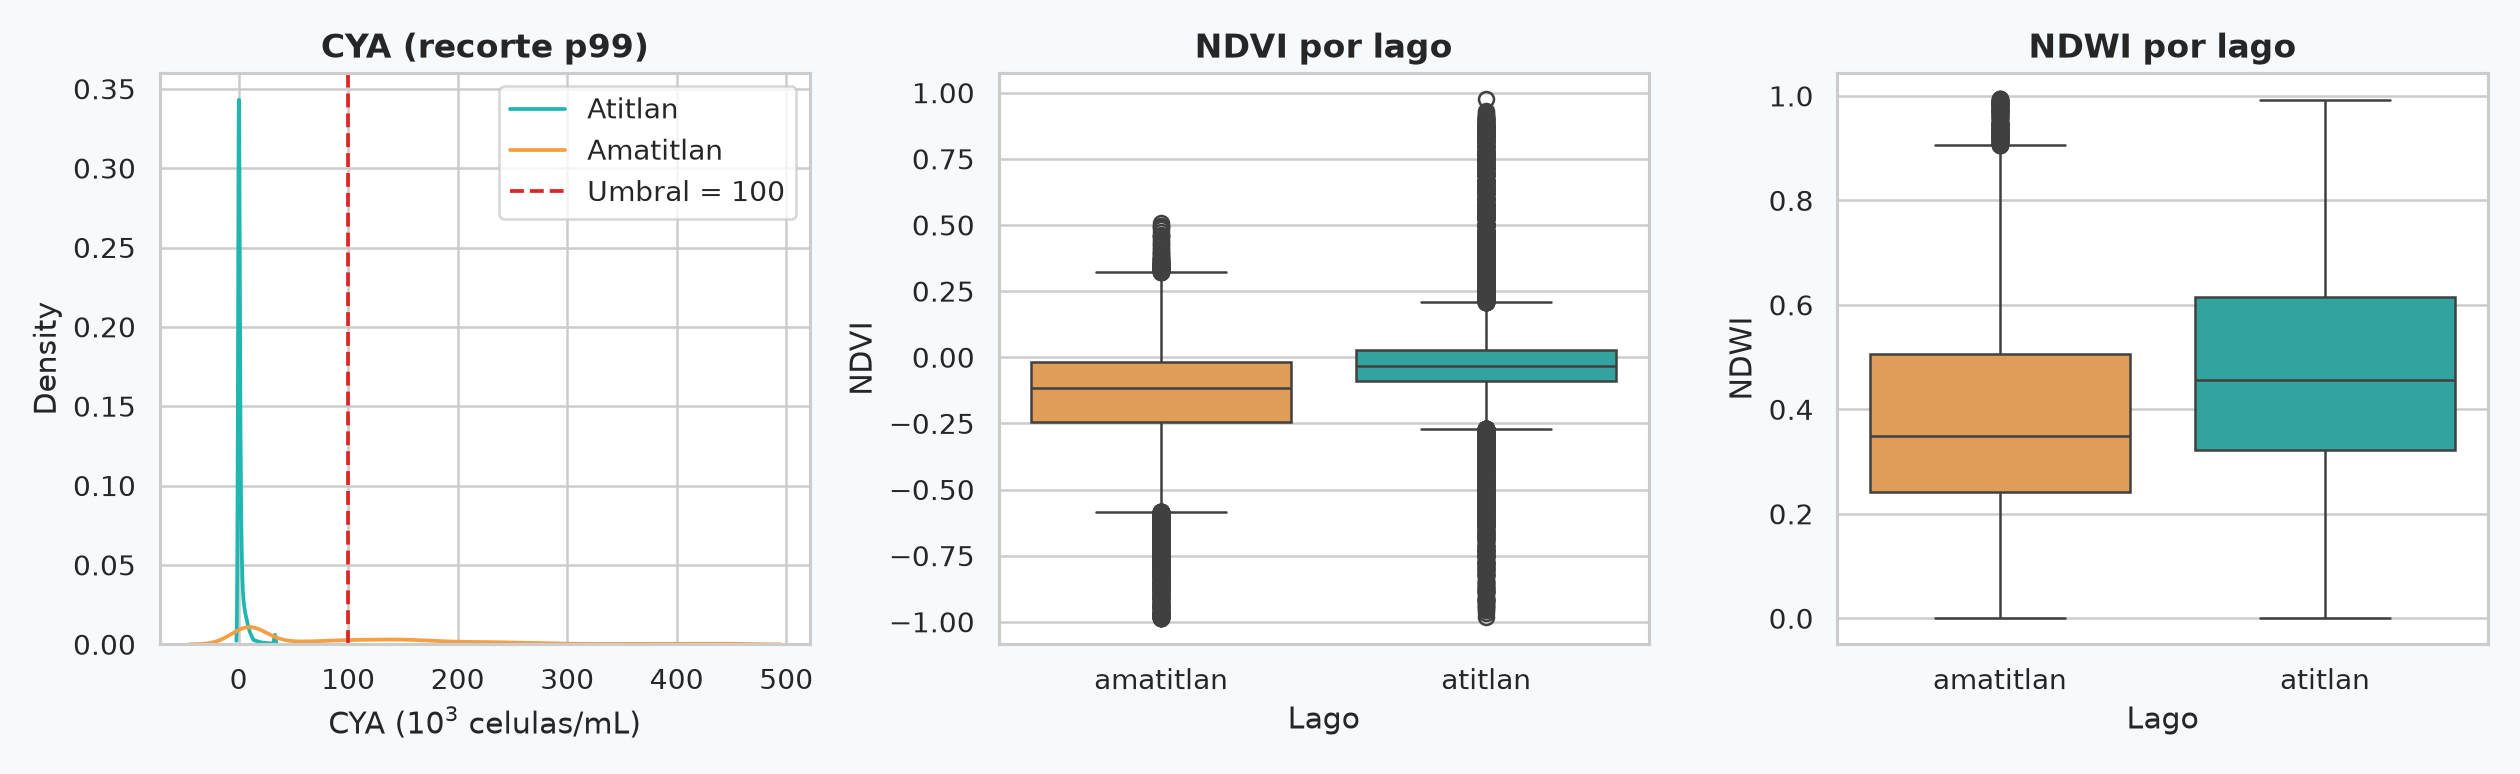
\includegraphics[width=0.78\textwidth]{ml_eda_indices_cya.png}
\caption{Exploración de CYA, NDVI y NDWI en la muestra reproducible.}
\end{figure}

\section{Respuesta binaria y desbalance}

Se definió $Y=1$ (concentración alta) cuando \cya{} $\geq 100$, equivalente a 100 000 células/mL. La referencia ambiental es el nivel histórico de alerta moderada de la OMS para agua recreativa. Se usa únicamente como umbral de cribado: Se2WaQ es una estimación óptica transferida y no una medición microscópica, taxonómica o toxicológica. Por tanto, una predicción alta debe motivar verificación in situ y no interpretarse como diagnóstico sanitario.

\begin{table}[H]
\centering
\caption{Distribución completa de la respuesta.}
\begin{tabular}{lrrr}
\toprule
Lago & Baja & Alta & Alta (\%)\\
\midrule
Atitlán & 3 030 910 & 10 842 & 0.36\\
Amatitlán & 215 849 & 161 455 & 42.79\\
\bottomrule
\end{tabular}
\end{table}

\begin{figure}[H]
\centering
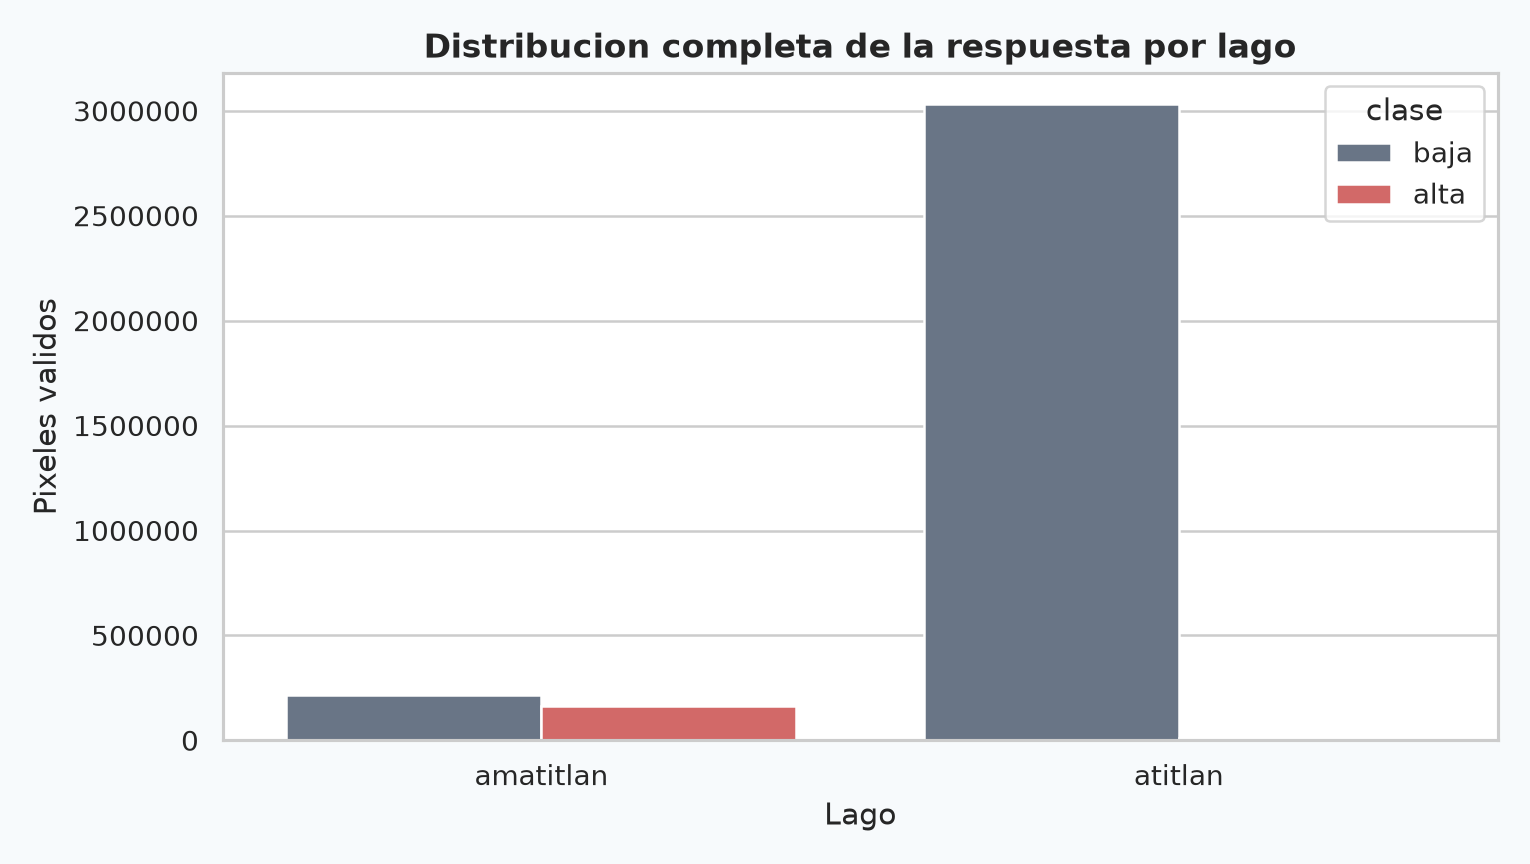
\includegraphics[width=0.66\textwidth]{ml_distribucion_clases.png}
\caption{Desbalance marcado y heterogéneo entre lagos.}
\end{figure}

La diferencia de prevalencias hace que accuracy sea insuficiente: un clasificador trivial podría parecer excelente en Atitlán. Por ello se reportan precision, recall, F1 y ROC-AUC. Desde vigilancia ambiental se prioriza recall, porque un falso negativo omite una zona potencialmente problemática; un falso positivo incrementa muestreo y costos, pero permite confirmación de campo.

\section{Predictores e ingeniería de variables}

La ecuación Se2WaQ usada en la Parte 1 es $115530.31[(B03\,B04)/B02]^{2.38}$. La Tabla~\ref{tab:leakage} documenta la exclusión estricta de variables con fuga.

\begin{table}[H]
\centering
\caption{Variables excluidas del entrenamiento.}
\label{tab:leakage}
\begin{tabularx}{\textwidth}{>{\bfseries}lX}
\toprule
Variable & Motivo\\
\midrule
CYA & Variable continua que define directamente la etiqueta.\\
B02, B03, B04 & Entran directamente en la ecuación de CYA.\\
NDVI & Usa B04, que participa en la construcción de CYA.\\
NDWI & Usa B03, que participa en la construcción de CYA.\\
\bottomrule
\end{tabularx}
\end{table}

Los predictores espectrales seguros son B05, B06 y B07 (borde rojo), B08 y B8A (infrarrojo cercano) y B11/B12 (infrarrojo de onda corta). Se añadieron coordenadas normalizadas dentro de cada lago para representar estructura espacial sin usar la separación absoluta entre lagos, y seno/coseno del día del año para codificar estacionalidad circular. El lago no se utilizó como predictor, lo que hace más honesta la transferencia cruzada.

\section{Modelos y ajuste}

Se aplicó una partición estratificada convencional de 70\% entrenamiento y 30\% prueba. Dentro del entrenamiento, una búsqueda en rejilla con tres pliegues seleccionó hiperparámetros por ROC-AUC sobre un máximo de 50 000 filas. Después se reajustó cada modelo con todo el entrenamiento y se conservó el mismo test para comparar.

\begin{table}[H]
\centering
\caption{Mejor configuración por algoritmo.}
\begin{tabularx}{\textwidth}{lXr}
\toprule
Modelo & Configuración seleccionada & ROC-AUC CV\\
\midrule
Regresión logística & $C=10$, estandarización, pesos balanceados & 0.994\\
Random Forest & 120 árboles, profundidad libre, hoja mínima 2 & 0.998\\
Gradient Boosting & tasa 0.10, 31 hojas, 160 iteraciones & 0.998\\
\bottomrule
\end{tabularx}
\end{table}

\section{Evaluación aleatoria, espacial y temporal}

\begin{table}[H]
\centering
\caption{Métricas principales. GroupKFold espacial es el promedio de cinco pliegues.}
\small
\begin{tabular}{llrrrr}
\toprule
Validación & Modelo & Accuracy & Precision & Recall & F1 / AUC\\
\midrule
Aleatoria & Logística & 0.967 & 0.874 & 0.989 & 0.928 / 0.995\\
Aleatoria & Random Forest & 0.984 & 0.952 & 0.973 & 0.963 / 0.999\\
Aleatoria & Gradient Boosting & 0.981 & 0.930 & 0.987 & 0.957 / 0.999\\
\addlinespace
Espacial & Logística & 0.967 & 0.874 & 0.986 & 0.927 / 0.995\\
Espacial & Random Forest & 0.982 & 0.952 & 0.963 & 0.958 / 0.998\\
Espacial & Gradient Boosting & 0.979 & 0.927 & 0.981 & 0.953 / 0.998\\
\addlinespace
Temporal & Logística & 0.870 & 0.687 & 0.938 & 0.794 / 0.959\\
Temporal & Random Forest & 0.776 & 0.992 & 0.162 & 0.279 / 0.903\\
Temporal & Gradient Boosting & 0.850 & 0.816 & 0.561 & 0.665 / 0.908\\
\bottomrule
\end{tabular}
\end{table}

Gradient Boosting se seleccionó por el mayor ROC-AUC aleatorio y recall alto. Random Forest obtuvo el F1 aleatorio más alto por margen pequeño, pero su recall temporal cayó a 0.162: fue demasiado conservador ante las últimas fechas (Atitlán 2026-07-22 y Amatitlán 2026-06-19). La regresión logística resultó menos precisa pero mucho más estable en recall temporal. Esta tensión impide declarar un único algoritmo ``mejor'' sin especificar el objetivo ambiental.

\begin{figure}[H]
\centering
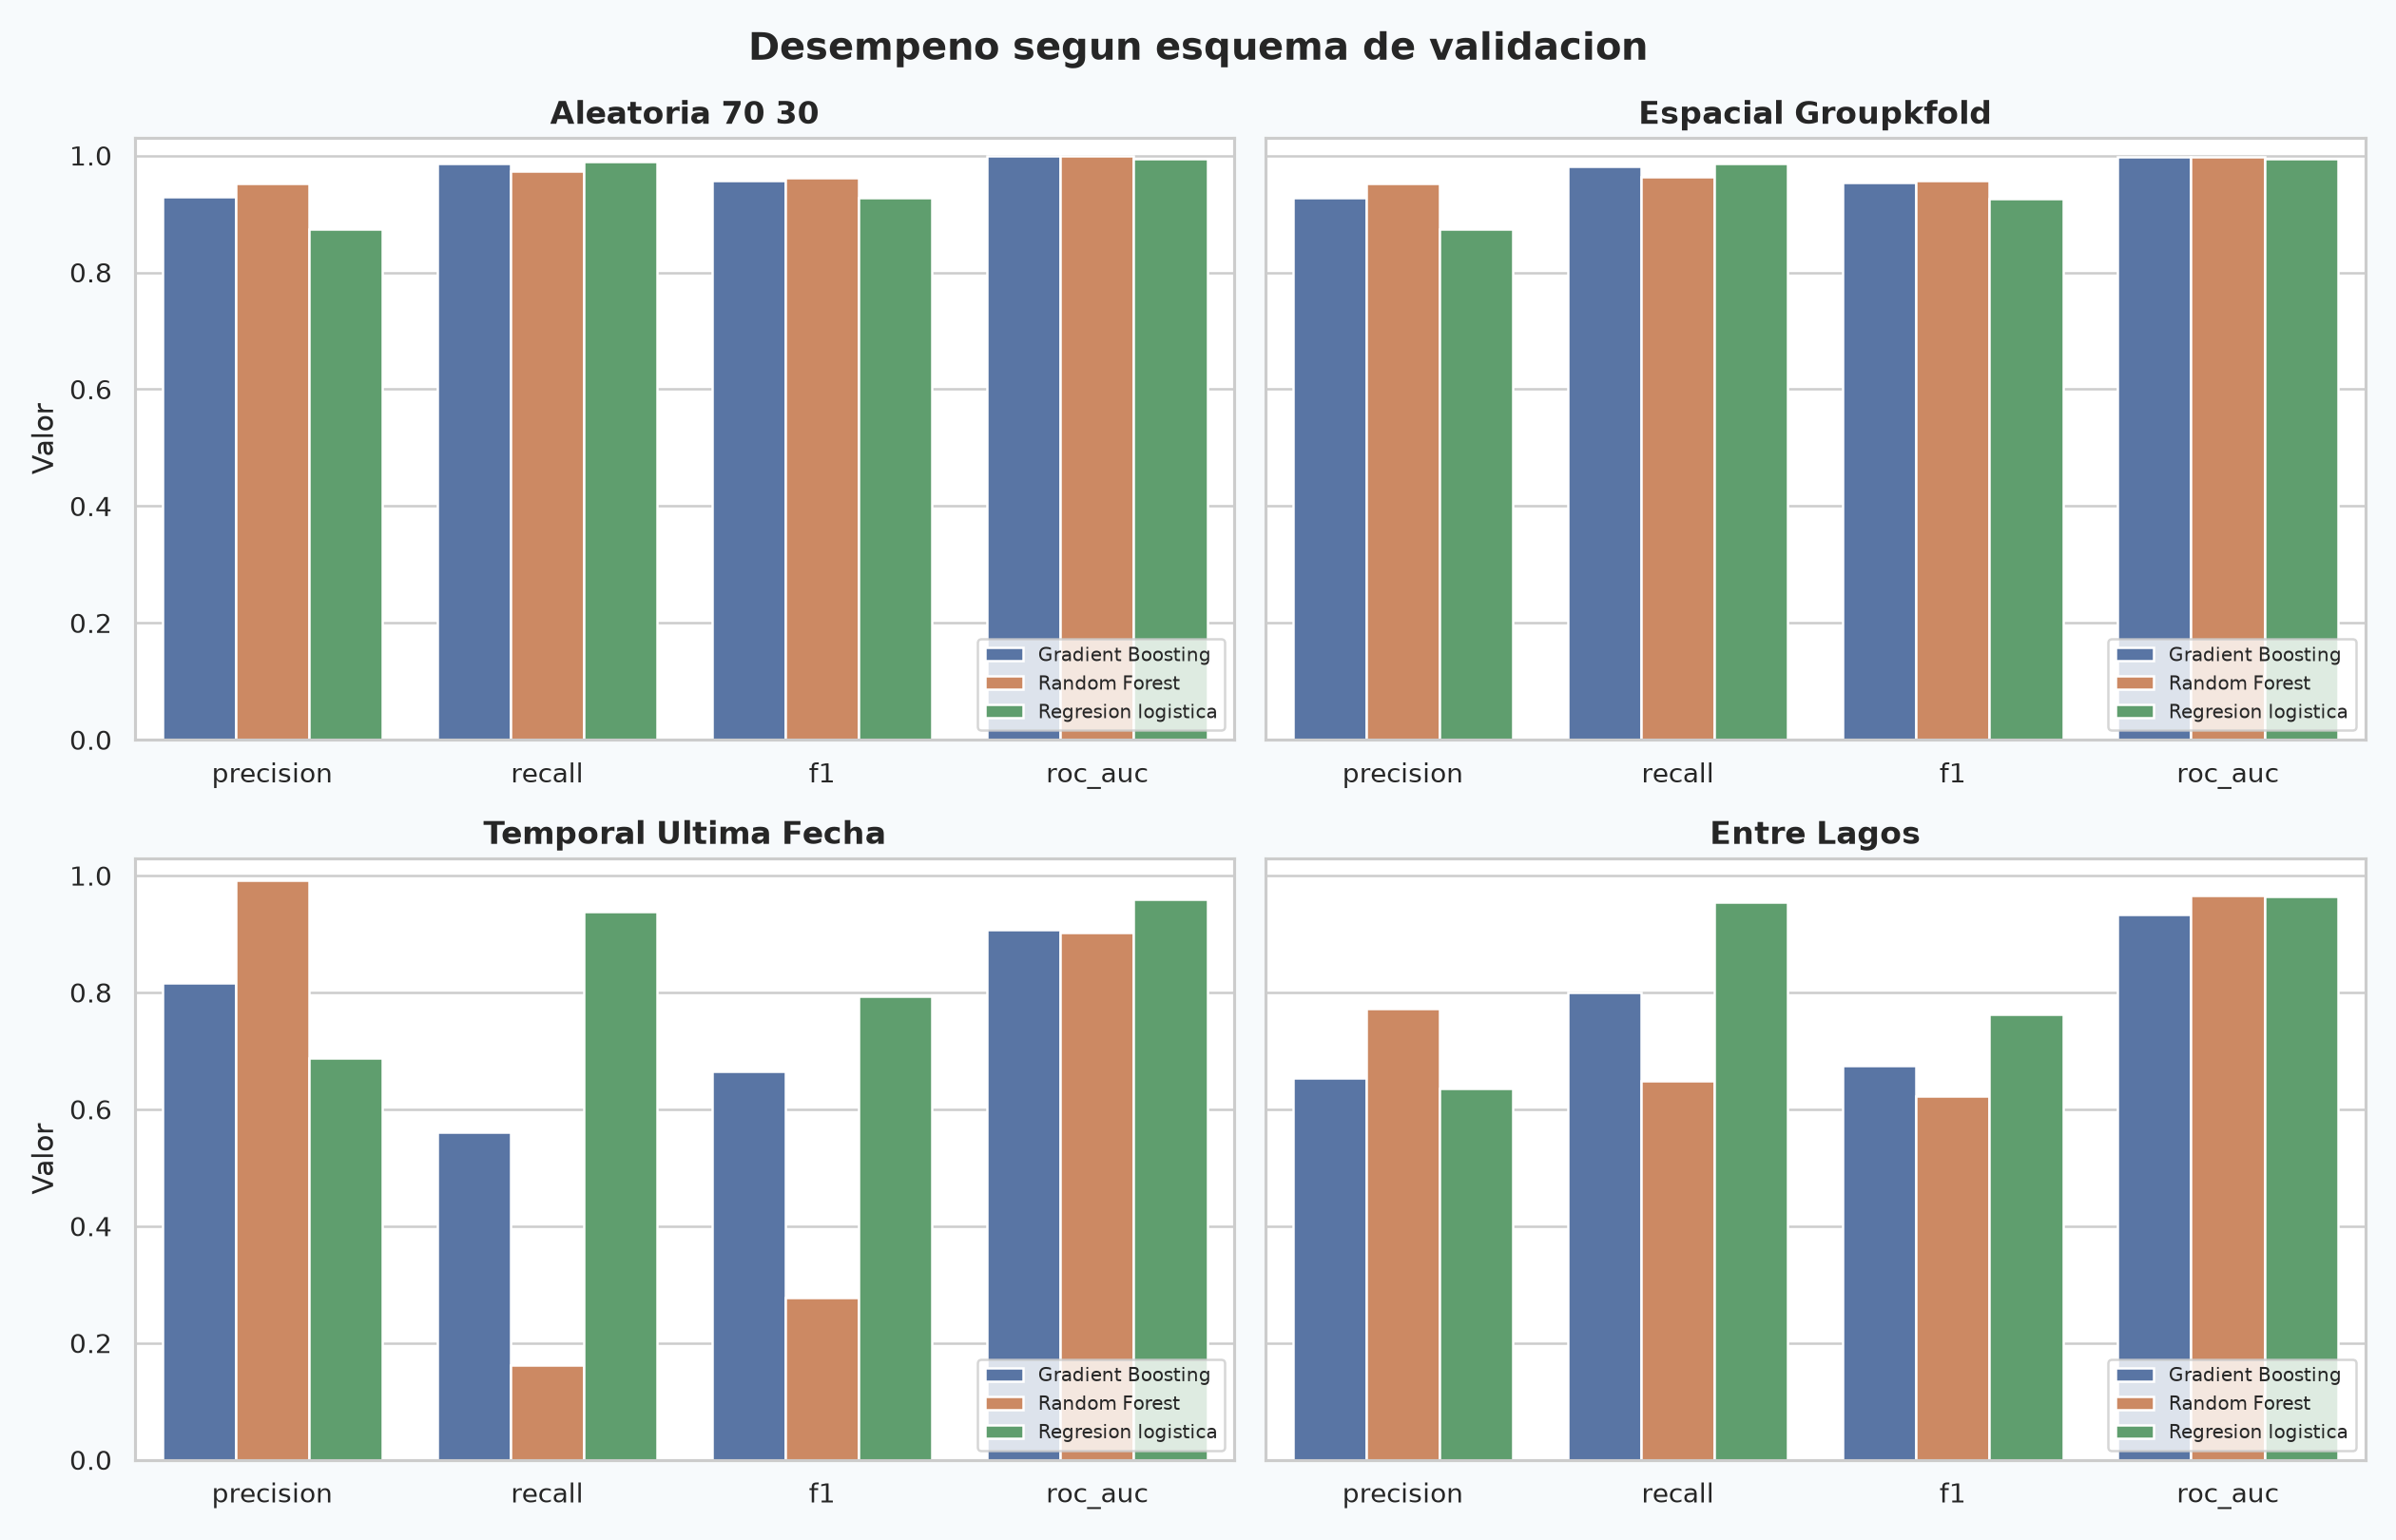
\includegraphics[width=0.96\textwidth]{ml_comparacion_validaciones.png}
\caption{La partición aleatoria sobreestima el comportamiento frente a cambio temporal y de lago.}
\end{figure}

\subsection{Validación espacial por bloques}

Las coordenadas se proyectaron a EPSG:32615 y se asignó cada píxel a una cuadrícula de 1 km. Se obtuvieron 167 bloques en Atitlán y 36 en Amatitlán. GroupKFold mantuvo todas las fechas de un mismo bloque exclusivamente en entrenamiento o prueba, evitando que el mismo lugar reapareciera en ambos conjuntos.

\begin{figure}[H]
\centering
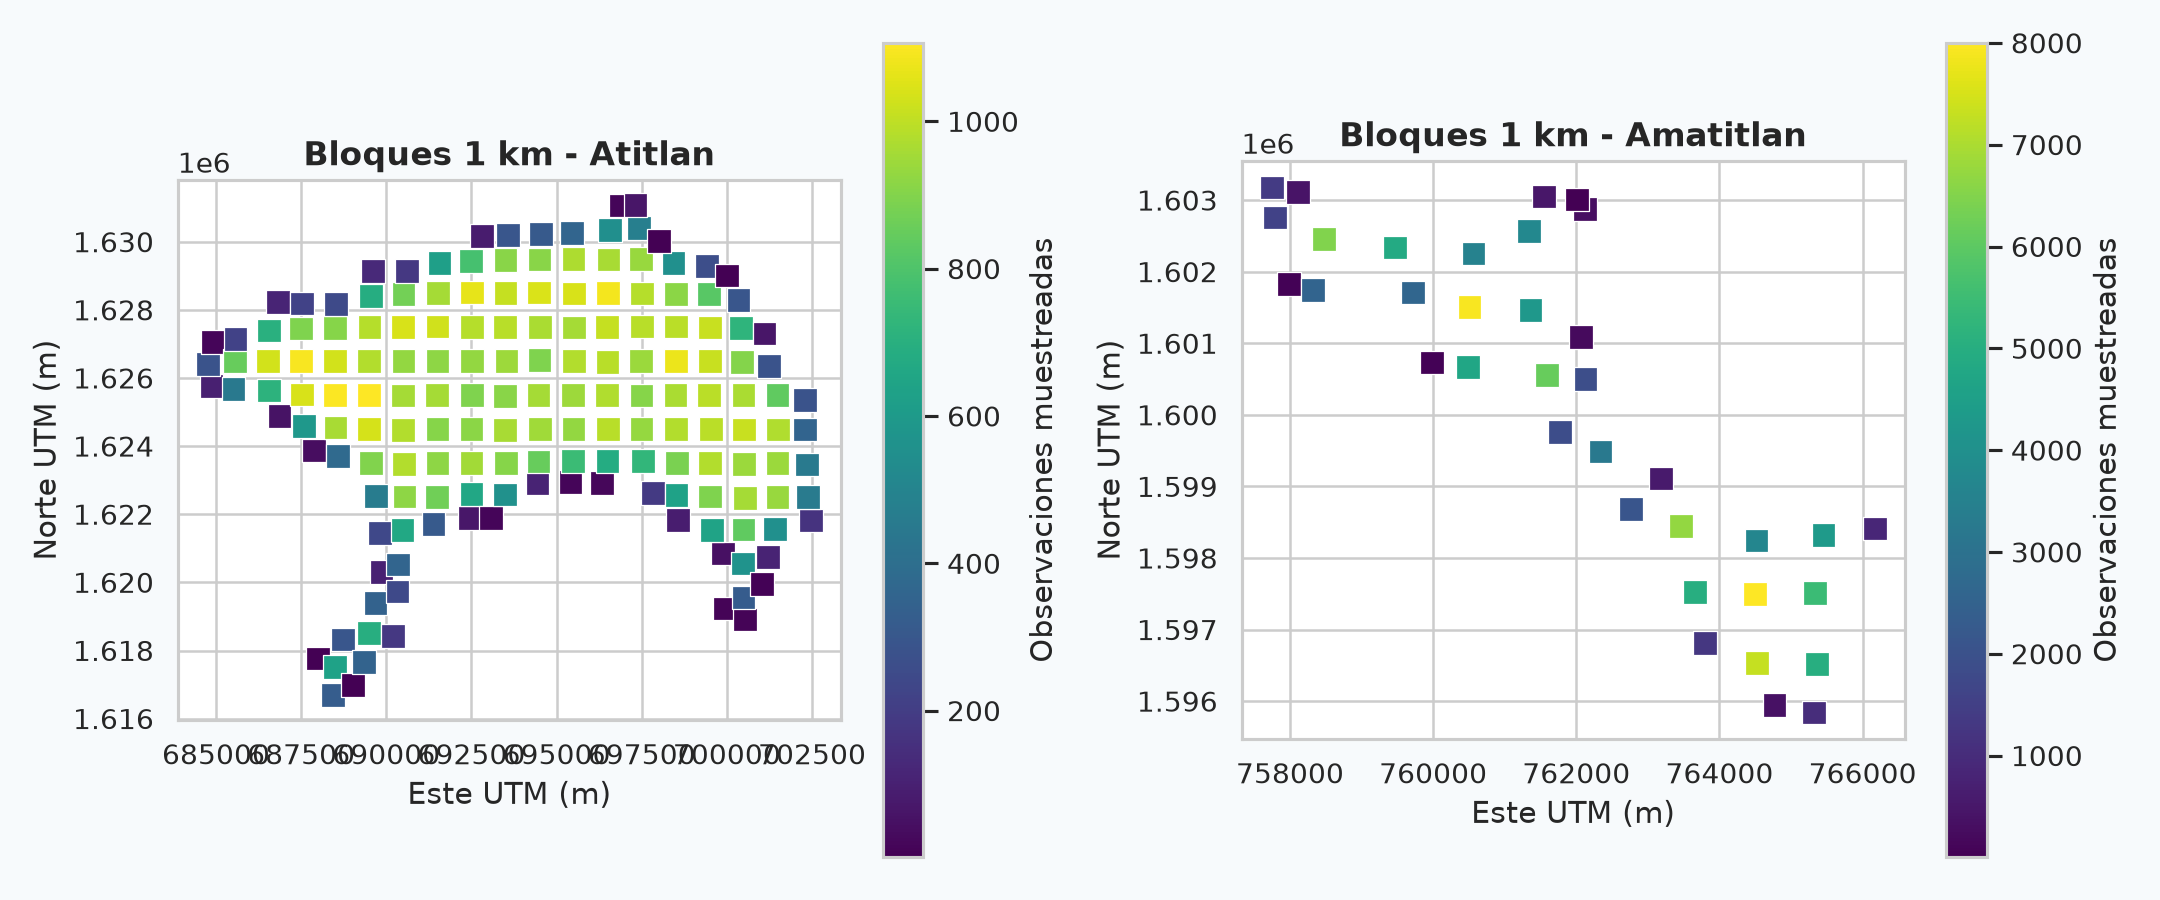
\includegraphics[width=0.92\textwidth]{ml_bloques_espaciales_1km.png}
\caption{Centroides de los bloques espaciales y cantidad de observaciones muestreadas.}
\end{figure}

Las métricas espaciales fueron cercanas a las aleatorias, lo que sugiere que las bandas independientes contienen señal transferible entre bloques. Sin embargo, GroupKFold reparte bloques no contiguos entre pliegues y conserva vecindad entre bloques adyacentes; en el corte final conviene contrastar además particiones espaciales contiguas si el presupuesto computacional lo permite.

\section{Transferencia entre lagos}

\begin{table}[H]
\centering
\caption{Prueba cruzada: entrenamiento en un lago y evaluación en el otro.}
\small
\begin{tabular}{llrrrr}
\toprule
Dirección & Modelo & Precision & Recall & F1 & ROC-AUC\\
\midrule
Atitlán $\rightarrow$ Amatitlán & Logística & 0.691 & 0.960 & 0.804 & 0.930\\
 & Random Forest & 0.964 & 0.364 & 0.529 & 0.938\\
 & Gradient Boosting & 0.865 & 0.658 & 0.747 & 0.869\\
\addlinespace
Amatitlán $\rightarrow$ Atitlán & Logística & 0.580 & 0.951 & 0.721 & 0.998\\
 & Random Forest & 0.580 & 0.932 & 0.715 & 0.994\\
 & Gradient Boosting & 0.441 & 0.943 & 0.601 & 0.999\\
\bottomrule
\end{tabular}
\end{table}

La generalización es asimétrica. Atitlán tiene apenas 0.36\% de positivos reales, por lo que entrenar allí limita la diversidad de episodios altos y reduce el recall en Amatitlán para los árboles. En sentido inverso, los modelos reconocen la mayoría de positivos escasos de Atitlán, pero con precisión moderada: numerosos espectros son marcados como altos en un lago donde la prevalencia es mínima. Las diferencias de profundidad, mezcla, altitud, cuenca y presión urbana hacen que un umbral espectral aprendido en un lago no sea automáticamente transportable.

\section{Importancia global preliminar}

La importancia por permutación del Gradient Boosting se calculó sobre una muestra independiente del test. B05 produjo la mayor caída de ROC-AUC (0.266), muy por encima de B08 (0.008) y la posición norte normalizada (0.005). B05 se ubica en el borde rojo, una región sensible a pigmentos y cambios ópticos de biomasa. Esta asociación es predictiva, no causal; materia suspendida, profundidad y condiciones atmosféricas pueden producir respuestas parecidas.

\begin{figure}[H]
\centering
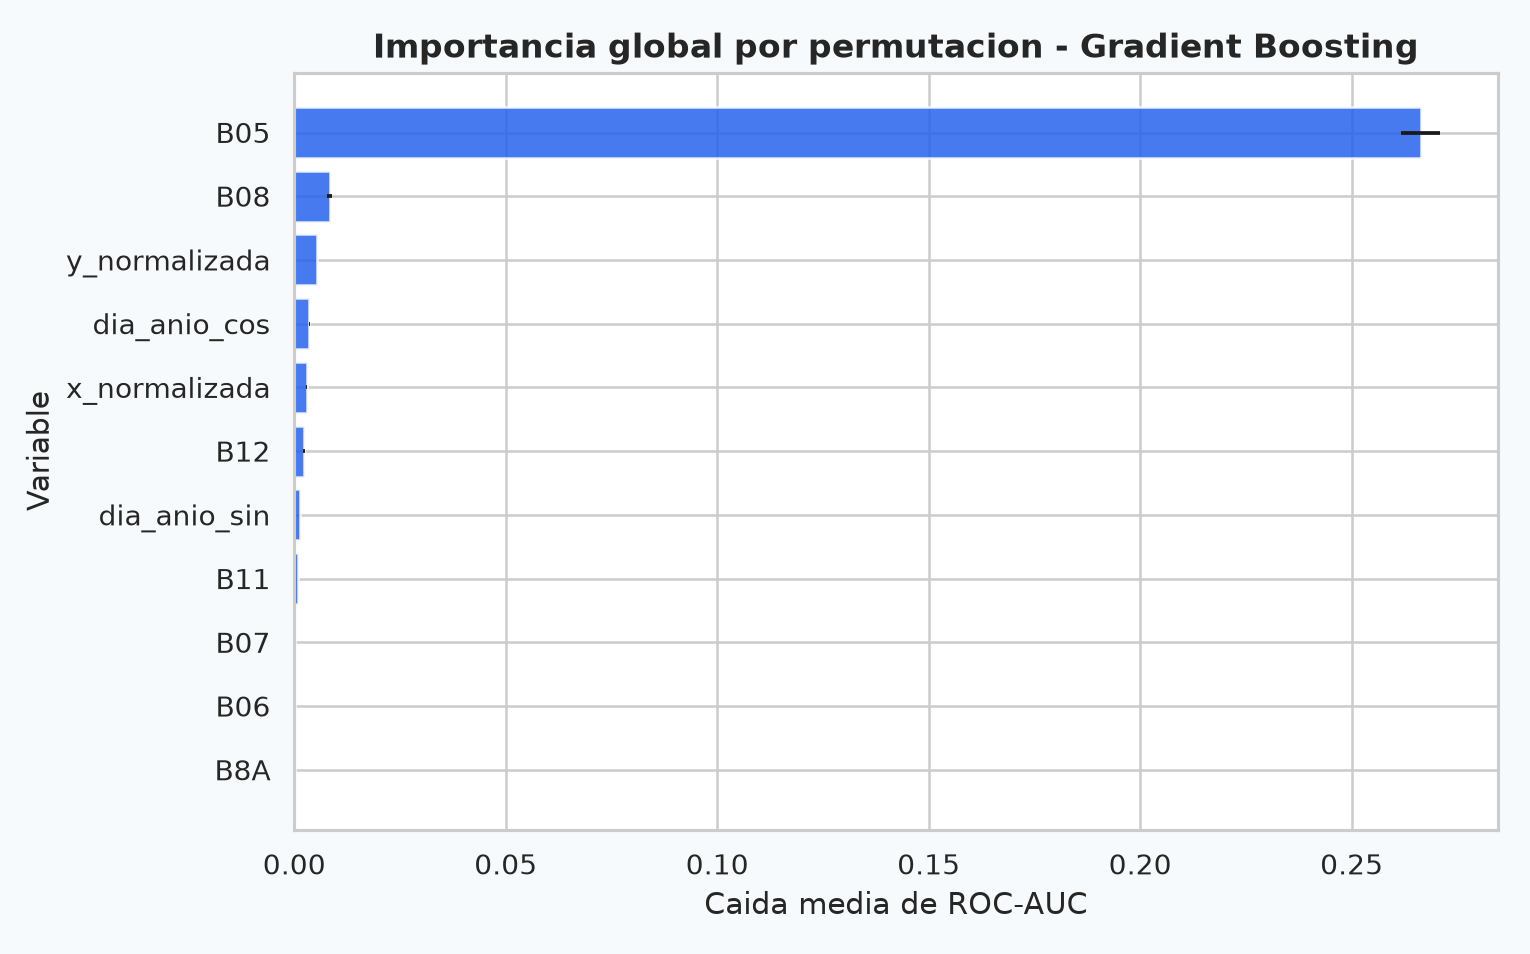
\includegraphics[width=0.72\textwidth]{ml_importancia_global.png}
\caption{Importancia global por permutación del modelo seleccionado.}
\end{figure}

\section{Conclusiones preliminares y trabajo restante}

El avance demuestra que es posible clasificar el proxy CYA con bandas no usadas en su construcción y obtener alta discriminación bajo validación aleatoria y espacial. La caída temporal y la transferencia asimétrica son resultados centrales: un modelo operativo requiere seguimiento de cambio de distribución y calibración local. Para vigilancia, la regresión logística ofrece el recall temporal más seguro; Gradient Boosting ofrece el mejor balance global en el corte actual.

El 25\% final comprenderá:
\begin{enumerate}
\item SHAP global y local, con dirección y magnitud de efectos;
\item mapas por lago de probabilidad y categorías de riesgo;
\item mapas de falsos positivos y falsos negativos, comparados con la Parte 1;
\item conclusiones definitivas, limitaciones, propuesta de muestreo in situ y datos adicionales.
\end{enumerate}

\section*{Referencias}

\begin{enumerate}
\item World Health Organization. \emph{Guidelines on recreational water quality: Volume 1, coastal and fresh waters}. 2021. \url{https://www.who.int/publications/i/item/9789240031302}
\item U.S. Environmental Protection Agency. \href{https://www.epa.gov/habs/world-health-organization-who-1999-guideline-values-cyanobacteria-freshwater}{\emph{WHO 1999 Guideline Values for Cyanobacteria in Freshwater}.}
\item Sentinel Hub. \emph{Se2WaQ -- Sentinel-2 Water Quality}. \url{https://custom-scripts.sentinel-hub.com/custom-scripts/sentinel-2/se2waq/}
\item Copernicus Data Space Ecosystem. \emph{openEO API}. \url{https://openeo.dataspace.copernicus.eu/}
\end{enumerate}

\end{document}
